\chapter{%
序論}

% 章アブストラクト
配管は気体、液体、粉粒対などの流体を輸送や配線の保護などを目的とする管のことである。
配管は様々な場面で使用されており、電気配線やケーブルを保護する電気配管や、生活に必要な水を家庭や学校などに輸送する水道管などが挙げられ、私達の生活において重要な役割を担っている。
そのため、配管を運用するにあたって常に耐久性と安全性を保ち続ける必要性がある。 \\

\section{研究背景}
BIM とは、Building Information Modeling の略称で、建築物や土木構造物などの情報をコンピュータ上に現実と同じ建物の立体モデルを
形成し、設計から維持管理までのプロセスをデジタル化する新しいワークフローの一環である。このBIMモデリングはこれまでの3Dモデリングとは
大きく異なる。まず、従来の3次元モデリングでは2次元上で作成した図面を元に、3次元の形状を形成し組み立てる手法であった。
そのため、3Dモデルに修正箇所があった際に、2次元の図面を全て修正してから再度構築する必要があり大きな手間が生じていた。
しかし、このBIM手法は一つのデータを修正すると全てのデータが連動し、関係する図面の該当箇所が自動修正され、従来の3Dモデリングよりも高校率で作業を行うことが可能になる。\\
 配管は建築物の中でも日常生活に欠かせない存在である。配管は生活に必要な物資を運用したり保護する役割があり、常に安全性と耐久性を満たす必要がある。
その配管の図面を作成する際にはアイソメトリック(アイソメ)図と呼ばれる立体を斜めから見た視点で表示した等角図が用いられる。
このアイソメ図の最大の特徴が配管のルートを人目でイメージしやすくなることだ。設計図には平面図や立体図、系統図など
様々な種類の図面を使用するが、配管の場合、配管同士が複数にも重なり合っているため左右上下からの視点では見分けることが困難である。そのため、アイソメ図は図面を立体的に描画する手法を扱えるため、
配管のルートや交差する配管の前後関係をイメージしやすくなる。\\
\begin{figure}[htbt]
	\centering
	 \includegraphics[height=75mm]{aisome.eps}
	 \caption{アイソメ図の例}
	 \label{fig:f1}
\end{figure}

アイソメ図を取得するためにはこれまでにLight Detection and Ranging(LIDAR)センサーと呼ばれるレーザー光を使用して離れた場所にある物体の形状や距離を測定できるセンサーを使用していた。
RGB画像では距離情報を取得できないことから、3次元モデリングは比較的困難とされているがLIDARセンサーは距離情報を取得できることから、オブジェクトの奥行きを点群データとして扱えるようになる。
LIDARセンサーは3次元情報を取得できる点や測定範囲や精度が良いというメリットがあるが、その反面他のセンサーと比較すると高価であるというデメリットを抱えている。そのため、広く一般的に使用するためには
安価なセンサーでデータ収集し図面を作成できることが望まれる。このような背景から近年RGBカメラやRGB-Dカメラを用いたLIDARセンサーよりも安価な機器を用いた認識手法が研究されている。
その認識手法には近年、機械学習による物体検出と姿勢推定のタスクがコンピュータビジョンにおいて幅広く研究されている課題である。

\begin{figure}[htbt]
	\centering
	 \includegraphics[height=95mm]{flow.eps}
	 \caption{従来のアイソメ図取得方法}
	 \label{fig:f2}
\end{figure}

\section{既存研究}
機械学習による画像認識分野は画像に写る物体を識別し位置を特定する物体検出や画像の画素ごとに識別を行うセグメンテーション、オブジェクトの位置情報に加えて向きを推定する姿勢推定問題など様々な分野で研究がなされている。
物体検出は画像内で認識したいオブジェクトがどこに存在しているのかをバウンディングボックスを用いて検出するのが一般的である。
その代表的なモデルとしてYOLOを紹介する[10]。このモデルはほぼ同時期に発表されたFast R-CNNと同様に、物体検出に大きな影響を与えた[12]。Convolutional Neural Network(CNN)と呼ばれる畳み込みという操作を
加えたニューラルネットワーク構造を使用してオブジェクトを検出する。CNNの中には畳み込み層やプーリング層といったいくつかの個性的な機能を備えた層が含まれ、人手による作業を必要とせず得られた特徴をもとに領域を予測することができる。
YOLOの特徴は従来までは境界設定と物体検出を2段階に行っていた作業を一度に行うことで推定速度の高速化を行うことができた。図1.2にYOLOのネットワーク構造示す。\\
\begin{figure}[htbt]
	\centering
	 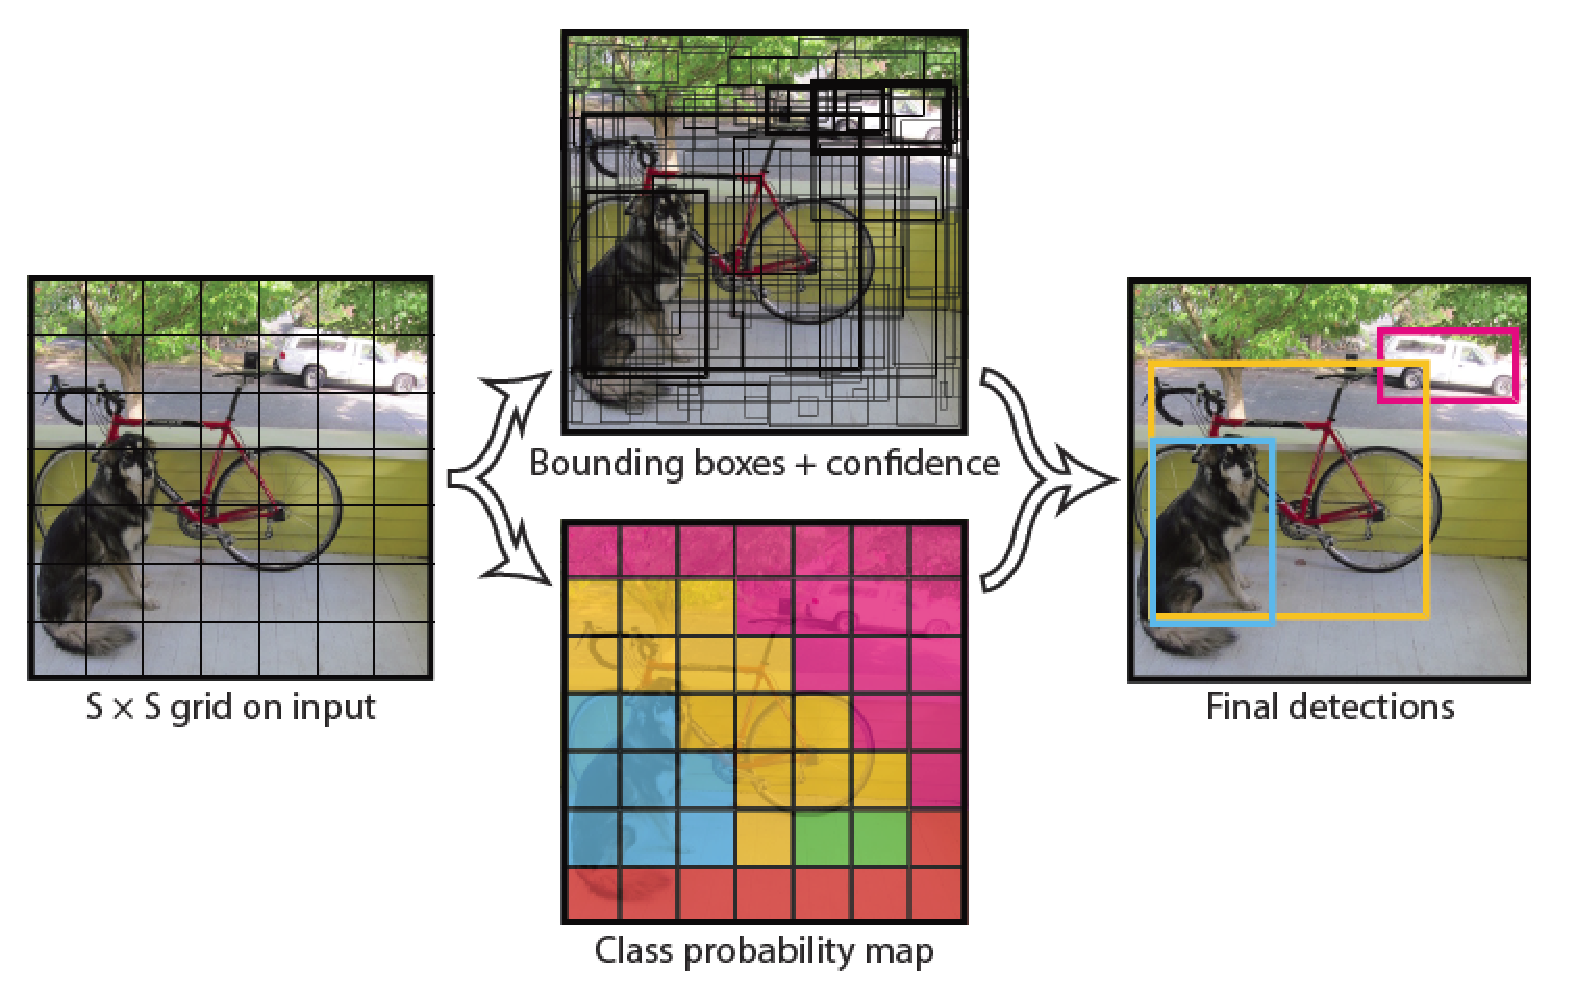
\includegraphics[height=75mm]{yolo.eps}
	 \caption{YOLOモデルの検出の流れ}
	 \label{fig:f2}
\end{figure}

まず、入力画像をS*Sのグリッドセルに分割し、各グリッドセルで複数個のバウンディングボックスと各バウンディングボックスの信頼度を計算する。
物体の中心がグリッドセルに存在していた場合に、そのセルが物体を検出するように学習する。次に、バウンディングボックスの推定では各グリッドセルにB個のバウンディングボックスを持ち、それらのボックスの信頼スコアを予測する。
信頼スコアとは背景ではなく物体が含まれている確率のことである。次に、各グリッドセルは複数のクラスに対する条件付き確率を予測する
算出された条件付きクラス確率と一つ前の個々のバウンディングボックスの信頼スコアを掛け合わせることで、バウンディングボックス毎の
クラスに対する信頼スコアを得ることができる。このスコアを使用しどのバウンディングボックスが正解の物体を推定しているのかを判断している。
これ以降、End-to-Endモデルと呼ばれる入力層から出力層まで全層の重みを一辺に学習する手法が物体検出の中で主流となった。\\
一般的な物体検出ではRGB画像を用いた手法が多いが、カラー画像にDepth画像を取り入れた物体検出方法も存在する。Depth画像は物体の奥行き情報や、外光の影響を受けづらいため暗闇の中でも安定してオブジェクトの特徴を捉えることができる点が優れている。
RGB-D画像を用いた物体検出はカラー画像と深度画像をそれぞれ両方畳み込みした値を最後の全結合層で結合するのみの手法が一般的であった[14]。しかし、この手法ではカラー画像と深度画像のそれぞれの特性を維持することはできず、最大限RGB-D画像の利点を活かすことができていなかった。
そこでSPnetモデルではクロス強化モジュール(CIM)を提案することでRGB画像と深度画像から抽出された特徴を維持したまま統合する機能を実現可能にした[13]。\\
次に、6D姿勢推定問題について紹介する。姿勢推定問題では物体検出と同様にRGBカメラやRGB-Dカメラを使用した推定方法がある。RGBカメラの姿勢推定問題では古典的な方法はキーポイントを検出し、既知のオブジェクトモデルを参照することによって推定する[1, 2, 3]。
また、最近の研究では2次元上でキーポイントを予測し[5]、PnPによって姿勢を算出することが可能になる[4]。また、画像からオブジェクトの姿勢を直接推定する手法も提案されている[6]。
RGB-Dカメラを用いた姿勢推定問題では奥行き情報を使用できるため参照できる情報量の増加により精度が向上している[7]。また、Densefusionは同様にRGB-D画像を用いて姿勢推定問題に取り組んだ[8]。
姿勢検出においてオクルージョンと呼ばれる手前にある物体が後ろにある物体を隠す問題が課題となっていたが、独自のネットワーク検出方法により、他のネットワークよりも優れた精度を示している。
6D姿勢推定を行うネットワークであるGeneralizable Model-Free 6-DoF Object Pose Estimation from RGB Images(Gen6D)を紹介する[9]。姿勢推定に必要な主なデータセットは
3次元データやカラー画像、深度データなどが代表的である。しかし、3次元データをデータセットに使用するには事前に、認識したいオブジェクトの3Dモデルを作る必要があるため、大きな手間が生じてしまう。
そのため、Gen6Dはデータセットに3Dデータを必要とせずカラー画像のみで物体の姿勢推定を行える手法を提案した。データセットにはColmapと呼ばれる2次元画像から3次元点群を再構築するために使用されるソフトウェアが用いられている[11]。
Colmapに使用される2D画像はオブジェクトを異なる視点から撮影された画像を複数枚利用することで3次元情報を復元することができ、その点群データを学習して物体の6D姿勢を推定する。\\
\begin{figure}[htbt]
	\centering
	 \includegraphics[height=55mm]{gen6d-network.eps}
	 \caption{Gen6Dネットワーク構造}
	 \label{fig:f2}
\end{figure}

Gen6Dのネットワーク構成について図3に示す。まず、Detectorと呼ばれる工程では参照画像の情報をもとに認識したいオブジェクトの領域を検出する。
次の工程である、SelectorではDetectorで得られた領域の画像と最も近い視点を持つ参照画像を複数枚ある中から1つ抽出する。
これは選択された参照画像の視点をテスト画像の視点とほぼ同様とみなし、誤差は生じますがオブジェクトのポーズの初期姿勢を形成する.
最後の工程では先程得られた姿勢の改良を試みる。まず、参照画像から近い視点の画像をさらに6枚選択し、全参照画像間の平均と分散を算出し、
初期に求められた姿勢の情報を改善して最終的な結果を予測する。この研究のメリットとしてRGB画像のみを用意することで物体の姿勢を推定できるため、
データセットの作成は非常に容易である。しかし、このGen6Dをしようするにあたって問題点が2つある。まず、一つ目にRGB画像は距離情報を持たないため、
物体のスケール情報を明示することはできない。2つ目は一度の推論で複数の物体の姿勢推定を行うことができない点である。\\
アイソメ図を作成するにあたって、配管同士の距離情報は必ず明示する必要がある。また、暗闇の状況下でも配管を認識可能にするために、本研究ではRGBカメラではなくRGB-Dカメラを使用し、Depth画像を活用したネットワーク設計を試みる。






\section{研究目的}
 本研究ではRGBDデータを使用した深層学習による配管6D姿勢推定を行い、RGBDカメラを用いることによる安価な機器での姿勢推定の実現を試みる.
また,既存のRGB画像のネットワークにDepth画像を組み込んだモデルを提案し、認識精度向上と推定速度の高速化を目標とする。
本研究の貢献は以下のようになる。まず一つ目は深層学習によるRGB画像とDepth画像を用いた物体検出ネットワーク(RXD)の提案である。
RGB画像とDepth画像からそれぞれ抽出された特徴を結合するRxDLayerを導入し、他のネットワークと比較しRXDネットワークの有効性を示した。\\
2つ目は既存の6D姿勢推定ネットワーク(Gen6D)の複数物体検出を可能にさせたことである。配管は単体ではなく複数の管が張り巡らされているため、複数の
認識を可能にする必要がある。RXDネットワークでは画像内部にある配管全てを網羅し、それぞれの物体の中心ピクセル座標とスケールを推定することができる。\\
3つ目は本研究の最終目的であるアイソメ図を作成するにあたっての必要不可欠な配管距離測定である。アイソメ図は配管の向きだけでなく、距離情報を図面に
示す必要がある。そのため、Depth画像を用いることでネットワークによって認識された情報をもとに、配管の距離情報を算出することを可能にした。

\section{本手引の構成}
 本論文の構成は以下のようになる。第一章では研究背景、既存研究、研究目的について述べる。研究背景では、
Building Information Modeling(BIM)についてや従来のアイソメ図の取得方法について述べる。
既存研究では、6D姿勢推定と物体検出のそれぞれのネットワークを紹介する。
研究目的では、本研究の目的及び貢献について述べる。\\
第2章では,データ収集から配管アイソメ図までの方法や流れについて説明する。また、RXDネットワークの提案と構造図について紹介する.
第3章では,データセットの概要について述べる。データセットを収集する機器についてやRGB-Dカメラを使用するに適した配管のデータセットについて紹介する。
第4章では,物体検出や姿勢推定をテスト画像の結果や評価指標に基づいた数値より考察する.
第5章は結言である.
